\documentclass[letterpaper, 11pt]{article}

\usepackage[top=0in, bottom=1in, left=1in, right=1in, includehead, includefoot]{geometry}
\usepackage[utf8]{inputenc}
\usepackage[english,russian]{babel}
\usepackage{titlesec}
\usepackage{xcolor}
\usepackage{graphicx}
\usepackage{wrapfig}
\usepackage{float}
\usepackage{hyperref}
\usepackage{amssymb}



\definecolor{headerColor}{HTML}{003300}
\renewcommand{\familydefault}{phv}

\titleformat{\section}[hang]
    {\Large}
    {\thesection}
    {0.3in}
    {}
    [\color{headerColor}\hrule height 0.5pt]



\begin{document}

    \begin{wrapfigure}{R}{0.25\textwidth}
        \centering
        \vspace{-5pt}
        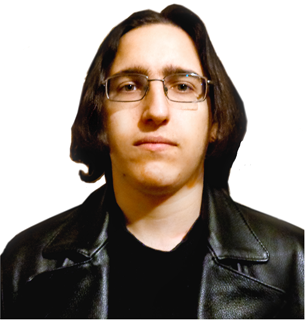
\includegraphics[width=0.25\textwidth]{src/images/pho_small_cut.png}
    \end{wrapfigure}

    \noindent
    \Huge
    Кивер Данила Андреевич \\
    \normalsize

    \noindent
    Контакты: danila.kiver@mail.ru или +7-909-645-38-84. \\

    \noindent
    Образование: МГУ имени М. В. Ломоносова, физический факультет, кафедра компьютерных методов физики, бакалавр. \\

    \noindent
    Коммуникация: upper-intermediate английский; есть опыт работы в распределенных командах (включая англоязычные). \\

    \noindent
    Публичные профили (кликабельно!): \href{https://stackoverflow.com/users/7191047/danila-kiver}{StackOverflow}, \href{https://unix.stackexchange.com/users/297621/danila-kiver}{Unix StackExchange}, \href{https://github.com/QazerLab}{GitHub}.





    \section{Опыт работы}

    Общий стаж --- 5 лет.

    \begin{itemize}
        \item
            Senior Software Engineer \\
            \footnotesize
                EPAM Systems, май 2018 -- декабрь 2019
            \normalsize
            
            \begin{itemize}
                \item
                    Проект PERF: мигрировал решение (Java-монолит на SpringBoot + PostgreSQL) в облако (VM с Ubuntu Server $\rightarrow$ GKE).
                \item
                    Проект Axway Syncplicity (\url{https://www.syncplicity.com}): разрабатывал и поддерживал бэкенд системы (message queue, content search, cloud storage) и сервисы, устанавливаемые on-premises (on-prem storage). Работал непосредственно с англоязычным заказчиком (включая ежедневные совещания и активную переписку). Технический стек --- Java-сервисы на SpringBoot + MariaDB на VM с CentOS 7 в AWS. Legacy-сервисы на Scala + Play.
                \item
                    Участвовал во внутренней программе менторинга в роли ментора.
                \item
                    Выступал на технических митапах, в т.ч. на внешнем (тема --- детали реализации Linux-контейнеров и используемые ими интерфейсы ядра).
            \end{itemize}

        \item
            Senior Software Engineer \\
            \footnotesize
                NetCracker Technology, апрель 2017 -- май 2018
            \normalsize
            
            \begin{itemize}
                \item
                    Разработал прототип системы Zero Touch Provisioning для проекта SD-WAN. Технический стек --- Java-сервисы на SpringBoot + PostgreSQL в OpenShift Origin.
                \item
                    Разработал и поддерживал отказоустойчивый облачный кластер PostgreSQL на базе фреймворка Patroni.
            \end{itemize}

        \item
            Software Engineer \\
            \footnotesize
                NetCracker Technology, ноябрь 2014 -- март 2017
            \normalsize

            \begin{itemize}
                \item
                    Мигрировал существующее решение (Java-монолит на WildFly + Spring + PostgreSQL) в облачное окружение (OpenShift Origin).
                \item
                    Участвовал в разработке и поддерживал отказоустойчивую инфраструктуру на базе Pacemaker.
                \item
                    Развивал и поддерживал низкоуровневые Java-библиотеки (persistence, history, platform abstraction) корпоративной платформы.
            \end{itemize}
    \end{itemize}





    \section{Sanity Check}

    \renewcommand{\labelitemi}{\checkmark}

    Без адекватной культуры разработки любой проект становится неподдерживаемым в кратчайшие сроки независимо от технической квалификации команды и используемых технологий и инструментов, поэтому я подтверждаю, что:

    \begin{itemize}
        \item Я уважаю принципы Twelve-Factor App и следую им.
        \item Я понимаю важность грамотного версионирования и ветвления. Я склонен к следованию SemVer и Trunk-based Development, но понимаю, что при наличии мотивации и пояснительной документации в команде могут быть использованы другие схемы версионирования и ветвления. 
        \item Я понимаю необходимость ревью кода и понимаю, что хорошее ревью возможно только для небольших изменений и при наличии внятных пояснений к PR/MR.
        \item Я понимаю, что CI/CD --- это подход к организации процесса разработки, а не конкретные инструменты и факт их использования сам по себе.
        \item Я понимаю идею DevOps и понимаю, что это культура и методология разработки, а не название выделенной команды из автоматизаторов / сетевиков / эникейщиков / релиз-инженеров / ... (place your DevOps anti-pattern here).
        \item Я понимаю, что по указанным выше причинам корректное применение практик CI/CD и DevOps невозможно без надлежащего майндсета в команде разработки, без понимания этой командой инфраструктуры под приложениями и процессов разработки.
    \end{itemize}
    
    \renewcommand{\labelitemi}{\textbullet}





    \section{Технические навыки}

    \begin{itemize}
        \item Linux (общий опыт --- 10+ лет с разными дистрибутивами, включая desktop; ``боевой'' опыт --- 5 лет на CentOS 6/7 и Ubuntu Server).
        \item Языки: Java 8 (основной язык), bash.
        \item Инфраструктура: Docker, OpenShift Origin до 3.6 (включая администрирование кластера) и Kubernetes, IaaS --- OpenStack (как пользователь) и AWS.
        \item SCM: Ansible, Salt.
    \end{itemize}





    \section{Околопрофессиональные интересы}

    Активно изучаю различные (альтернативные моему текущему техническому стеку) подходы и парадигмы в разработке (Rust, Haskell, C). Знакомлюсь с низкоуровневым устройством используемых технологий (изучаю код всего используемого стека --- в т.ч. Docker, Linux kernel, JDK/JVM; экспериментирую и ломаю всевозможными способами). \\

    \noindent
    По возможности разбираю интересные проблемы на StackOverflow и Unix StackExchange (ссылки на профили в шапке резюме). По мере необходимости выполняю мелкие исправления и улучшения в open-source проектах; не боюсь коммуницировать с коммьюнити.

\end{document}
